\documentclass{report}
\usepackage[utf8]{inputenc}
\usepackage{amsmath}
\usepackage{graphicx,float}
\usepackage{caption}
\usepackage{subcaption}
\usepackage{gensymb}
\usepackage[margin=1.25in]{geometry}
\usepackage[numbered,framed]{matlab-prettifier}
\usepackage{tikz}

\title{Sound Field Control with a Coaxial, Cardioid, Axisymmetric Loudspeaker}
\author{Alex Booth, supervised by Jonathan Hargreaves\\ a.booth9@edu.salford.ac.uk}

\begin{document}

%titlepage
\thispagestyle{empty}
\begin{center}
\begin{minipage}{0.75\linewidth}
    \centering
%University logo
    
\includegraphics[width=0.75\linewidth]{figs/Logo.jpg} \\
    \hrule
    \vspace{3cm}
%Thesis title
    {\uppercase{\Large Sound Field Control with an Axissymetric, Cardioid Loudspeaker\par}}
    \vspace{3cm}
%Author's 
    {\Large Alex Booth, supervised by Dr. Jonathan Hargreaves\par}
    \vspace{3cm}
%Degree
    {\Large A dissertation submitted for the degree of Audio and Acoustical Engineering BEng.\par}
    \vspace{3cm}
%Date
    {\Large May 2023}
\end{minipage}
\end{center}
\clearpage

\chapter*{Declaration}

\chapter*{Abstract}
    \textit{}

\chapter*{Dedication}



\chapter*{Acknowledgements}

\tableofcontents
\newpage

\chapter{Introduction}
    The Audio Engineering Society (AES) defines sound field control as the `process of creating a set of loudspeaker signals to create a certain listening experience over a listening area' \cite{AESsoundfieldcontrol}.
    The directionality of a loudspeaker can be a definitive tool of active sound field control; directional configurations, such as line arrays or subwoofers arranged to give cardioid directivity, are commonplace in live entertainment.

    An axisymmetric, cardioid loudspeaker has been constructed by Jonathan Hargreaves in association with students at the Universtiy of Salford.
    This loudspeaker consists of a perspex cylindrical two-driver coupled cabinet with drivers mounted at either end of the cylinder, and a KEF Uni-Q mid-high driver mounted coaxially with the `front' end of the cylindrical body.
    A diagram of the system is give in Fig.SPEAKER DIAGRAM.


    RESEARCH PROBLEM
    The main goal of the work described in this paper was to bring the axisymmetric, cardioid loudspeaker (ACL for the rest of this paper) into a physical testing environment, and from that testing environment, determine suitable signal processing to achieve optimal low-frequency cardioid directivity.
    Attention was paid to previous work on the ACL, and facets of this previous work informs the signal processing investigated in this report.
    SIGNIFICANCE
    Once the ACL is brought to a working stage by this project, further investigation into it's suitability for sound field control and other applications can take place.

    LIMITATIONS
    The described project is one in a more numerous collection of student works on this ACL, and as so these works are somewhat fragmented.
    Furthermore, the precise directivity predicted to be achieved by this loudspeaker may not have any current practical applications maybe?????

    STRUCTURE

    THE SPEAKER ITSELF AND HOW EACH DRIVER PERFORMS



\chapter{Literature Review}
    AUTHOR'S PROBLEM
    KEY CONCEPTS IN SOURCE
    KEY THEORIES
    DO THEY INNOVATE OR REFINE?
    CONCLUSIONS?
    HOW DOES IT RELATE TO OTHER LITERATURE?
    STRENGTHS?
    WEAKNESSES?

    \section{Sound Field Control}
        

    \section{Applications of Sound Field Control}

        Outdoor sound field control is commonplace practiced at major outdoor audiovisual events.
        Controlling the directivity of sound at an outdoor event is vital to both ensure even distribution of experience to an audience, and isolation of neighbors from noise pollution.
        Franz M. Heuchel, Diego Caviedes-Nozal, Jonas Brunskog, et al\. explore this in their paper: `Large-scale outdoor sound field control' \cite{heuchel2020large}.
        The authors investigate the low-frequency directivity performance of loudspeaker systems across atmospherically varying outdoor spaces, as opposed to the linear, homogenous, isotropic indoor conditions described in OTHER PAPERS.
        Wave field synthesis is a particular technique of sound field control, where arrays of loudspeakers 

    \section{Directional Loudspeakers}



        Harry Olson's `Gradient Loudspeakers'~\cite{olson1973gradient} forms the theoretical foundation of controlling the directionality of emitted sound with multiple loudspeaker drivers.
        The key concept Olson introduces is the `gradient loudspeaker', which are organized into orders.
        Zero-order gradient loudspeakers utilize a single driver within a sealed cabinet to give a theoretical monopole directionality, much like an omnidirectional microphone.
        Higher orders introduce directionality; a first-order unidirectional loudspeaker constructed with a spaced and delayed pair of zero-order gradient speakers operating 180\degree\@ out of phase gives a cardioid response.
        The delay between both drivers is fixed across all frequencies.
        Olson gives the radiated pressure of this unidirectional gradient loudspeaker, shown in Eq.\ref{olsonFirstOrderPressure}.
        \begin{equation}
            p = 2CU_f\cos{kct}[\sin{\frac{kd}{4}+\frac{kD}{4}\cos{\theta}}]
            \label{olsonFirstOrderPressure}
            \cite{olson1973gradient}
        \end{equation}
        \begin{figure}[H]
            \centering
            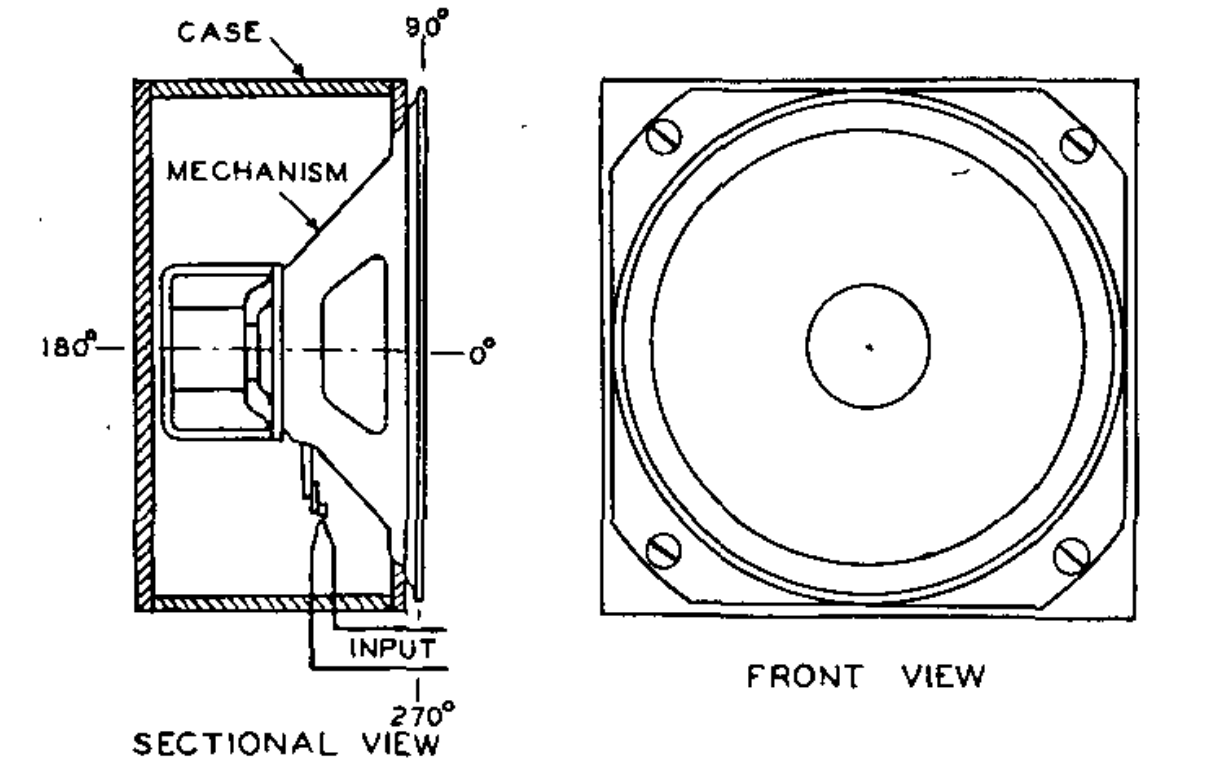
\includegraphics[scale=0.2]{figs/olsonFirstOrder.png}%
            \caption{Olson's first order unidirectional loudspeaker.}\cite{olson1973gradient}
            \label{olsonFirstOrderDiagram}
        \end{figure}
        Olson states that if the distance between the drivers, $D$ equals $d$, the distance delay introduced and seen in Fig.\ref{olsonFirstOrderDiagram}, the directivity of the system will be cardioid.
        The wavenumber, $k$, found in Eq.\ref{olsonFirstOrderPressure}, introduces a frequency dependence to the $D=d$ condition, thus affecting how cardioid the speaker may be.
        
        \begin{figure}[H]
            \centering
            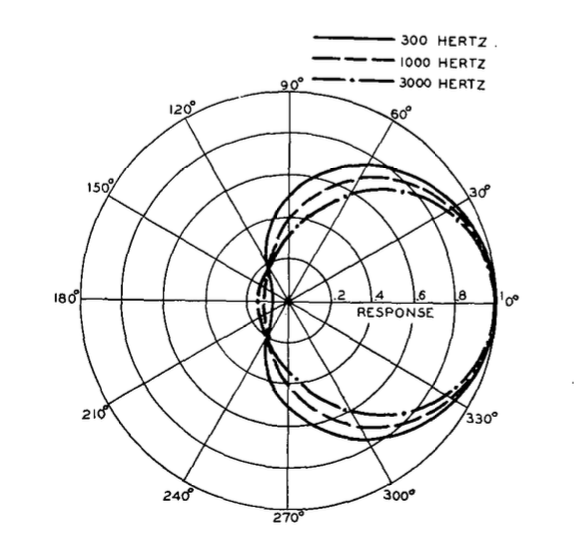
\includegraphics[scale=0.2]{figs/olsonFirstOrderDirectivity.png}%
            \caption{Olson's first order unidirectional loudspeaker.}\cite{olson1973gradient}
            \label{olsonFirstOrderDirectivity}
        \end{figure}


        Predating his work on gradient loudspeakers, Olson was an early descriptor of the beam narrowing effect of loudspeaker line arrays \cite{olson1957acoustical}.
        Line arrays would go on to be a principle tool of sound field control in the modern day, but gradient loudspeakers are still, relative to line arrays, uncommon.
        Cardioid subwoofer systems used in live audio are common implementations of gradient loudspeaker designs.
        These subwoofers can be sold as gradient loudspeakers themselves, often with switchable directivity patterns; audio engineers will also arrange standard, omnidirectional subwoofers into configurations that introduce a phase delay sufficient to create a cardioid directivity pattern~\cite{curtis2022cardioidsubs}.
        Jordan Cheer elaborates on the use of a `two source line array', which in essence is an Olson-style directional gradient loudspeaker, stating: `Two-source line arrays have been used in a variety of applications to generate localised listening zones and have also been used as a constituent element of larger arrays to achieve sound field control more generally.'\cite{cheer2015robustness}.


    \section{Loudspeaker Construction}
        The prototype ACL has each low-frequency driver mounted in a shared, acoustically coupled enclosure.
        Robustness and efficiency of an acoustically coupled two-source superdirective array, an ICSV22 paper by Jordan Cheer, elaborates on the benefits of such a shared enclosure \cite{cheer2015robustness}.
        Cheer acknowledges how a superdirective array of loudspeakers have `high sensitivity to uncertainties in the assumed response of the system', and that regularization of the powered signal driving units in an array can improve the `robustness to uncertainty'.
        However, he further notes that these measures may limit the directivity of a such a system; counterproductive to the designed purpose of a superdirective array.
        Robustness and efficiency thus sets out to investigate the robustness of acoustically coupled two-source superdirective loudspeaker, as opposed to the previously investigated non-interacting directional loudspeakers.
        Cheer finds, using a two-port model of loudspeaker behavior and derived simulations, that an uncoupled two-source array is `more significantly affected by response uncertainties than the coupled array', and thus the coupled array is more robust, avoiding the need for regularization.
        \begin{figure}[H]
            \centering
            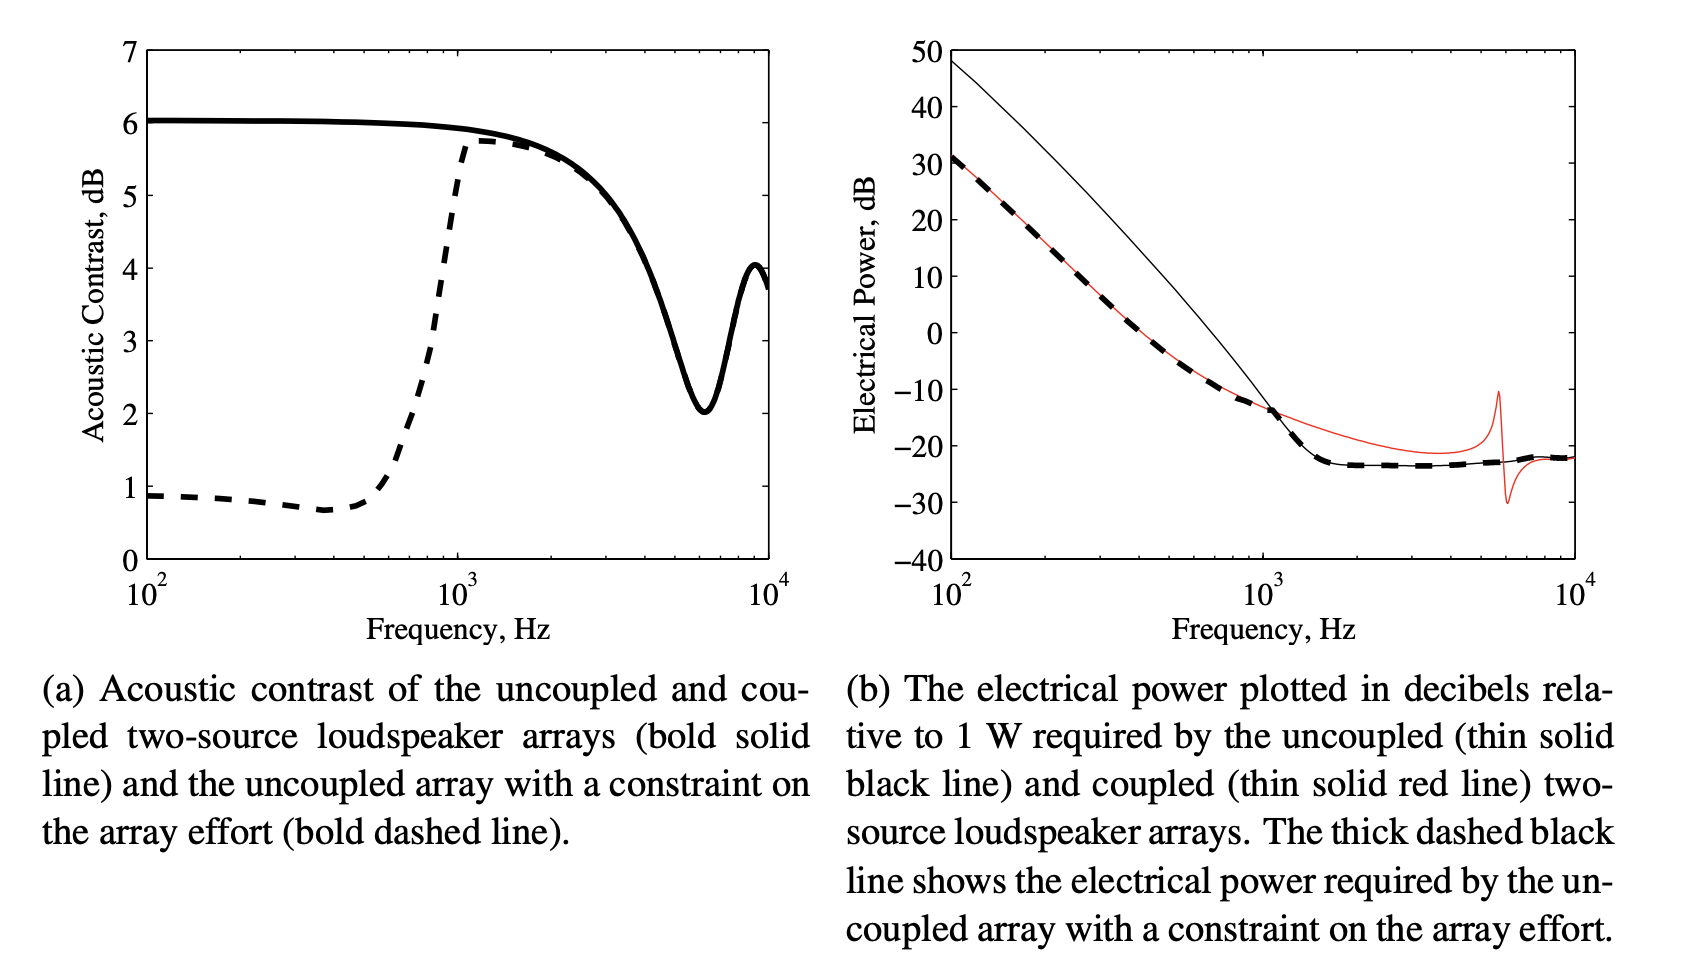
\includegraphics[scale=0.5]{figs/cheerGraph.png}%
            \caption{Cheer's plots comparing acoustically coupled and uncoupled loudspeaker systems.}\cite{cheer2015robustness}
            \label{cheerGraph}
        \end{figure}
        Cheer's figure \textit{a} (Fig.\ref{cheerGraph}) shows that when a constraint (to use the same electrical power as the coupled array) is applied to an \textit{un}-coupled two-source superdirective loudspeaker it loses a significant degree of acoustic contrast.

        SHAUN NIELSEN

        A BIT MORE HERE?
        Considering Cheer's findings, prior to the work this dissertation describes, the ACL was constructed with an acoustically coupled main chamber for the LF drivers.

        All the drivers used in the ACL are designed by KEF and used in their commercially available products, but in different cabinet configurations to the ACL.
        However, KEF have a commercialy available ceiling-mounted loudspeaker that utilizes an LF driver with a Uni-Q coaxially mounted: The Ci250RRM-THX.
        \begin{figure}[H]
            \begin{minipage}{.49\textwidth}
                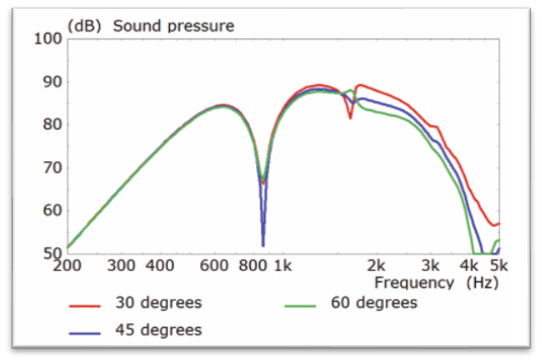
\includegraphics[width=\linewidth]{figs/KEFpressure.png}%
                \centering
                \caption{}
                \label{KEFpressure} \cite{KEFCi}
            \end{minipage}
            \begin{minipage}{.49\textwidth}
                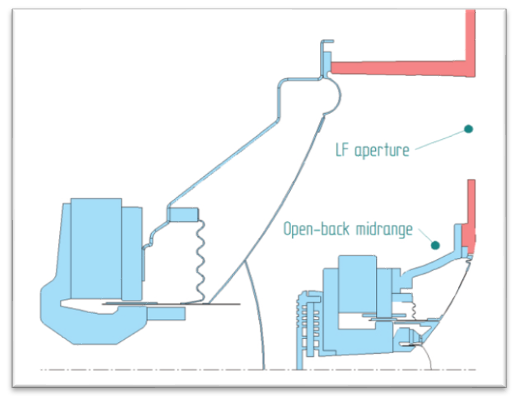
\includegraphics[width=\linewidth]{figs/KEFdiagram.png}%
                \centering
                \caption{ } \cite{KEFCi}
                \label{KEFdiagram}
        \end{minipage}
        \end{figure}
        KEF found that such a three-way loudspeaker design with the LF driver mounted in a cavity to the rear of the mid-high introduces resonances, determined by the size and shape of the cavity \cite{KEFCi}.
        Figure \ref{KEFpressure} shows a dip in sound pressure between 800Hz to 1KHz; KEF remedy this by designing the Ci250RRM-THX to use an open-backed Uni-q midrange.
        KEF call this `Cavity Radiation Control', and they show, in Fig. \ref{KEFopenback}, that the 30-plus dB cancellation around 800Hz to 1KHz is eliminated.
        \begin{figure}[H]
            \centering
            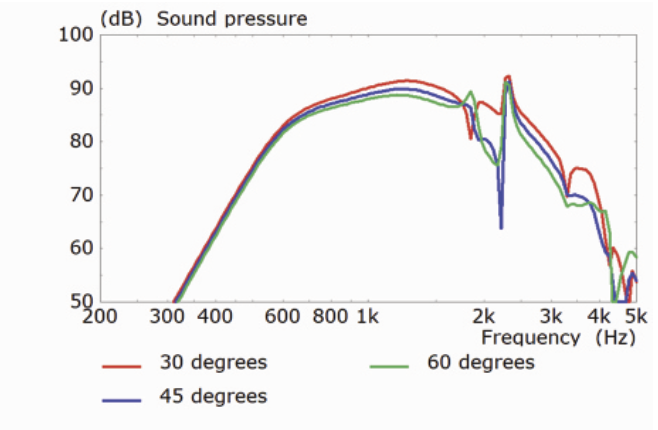
\includegraphics[scale=0.5]{figs/KEFopenback.png}
            \caption{Changing the Uni-Q to an open back design.}\cite{KEFCi}
            \label{KEFopenback}
        \end{figure}
        Whilst the model of LF driver and the cavity in which it is mounted in are different to the ACL, KEF's findings are applicable to the three-way coaxial design of the ACL and as such prompt further investigation into these `cavity resonances'.

    \section{Quantifying Loudspeaker Directivity} 
        When describing a new, `holographic' near-field method of loudspeaker directivity measurement, Wolfgang Klippel and Christian Bellmann elaborate on the use of spherical harmonics as constituent solutions to the Helmholtz equation \cite{klippel2016holographic}.
        Whilst their paper focuses on the holographic directivity measurement method's effectiveness at reducing the space requirements of anechoic listening environments, the description of spherical harmonics
        
        The project described in this dissertation builds on previous work not only by the supervisory but also by other (former) students of the University of Salford.
        During the COVID-19 lock-down period the acoustic properties of the prototype loudspeaker were modelled with computer simulations.
        Paul Vedier carried out these simulations as part of his Master's dissertation.
        A metric derived by Vedier, is used to quantify cardioid directivity and will be utilized to achieve the practical aims of correcting for cardioid directivity over all frequencies in the ACL.
        Vedier's paper confirms, using COMSOL, that the ACL has the properties of an Olson-style gradient loudspeaker.
        In Fig.\ref{vedierPolar} Vedier compares FEM analysis of two fully-modelled membranes in a cabinet and compares to Olson's analytical method.
        \begin{figure}[H]
            \centering
            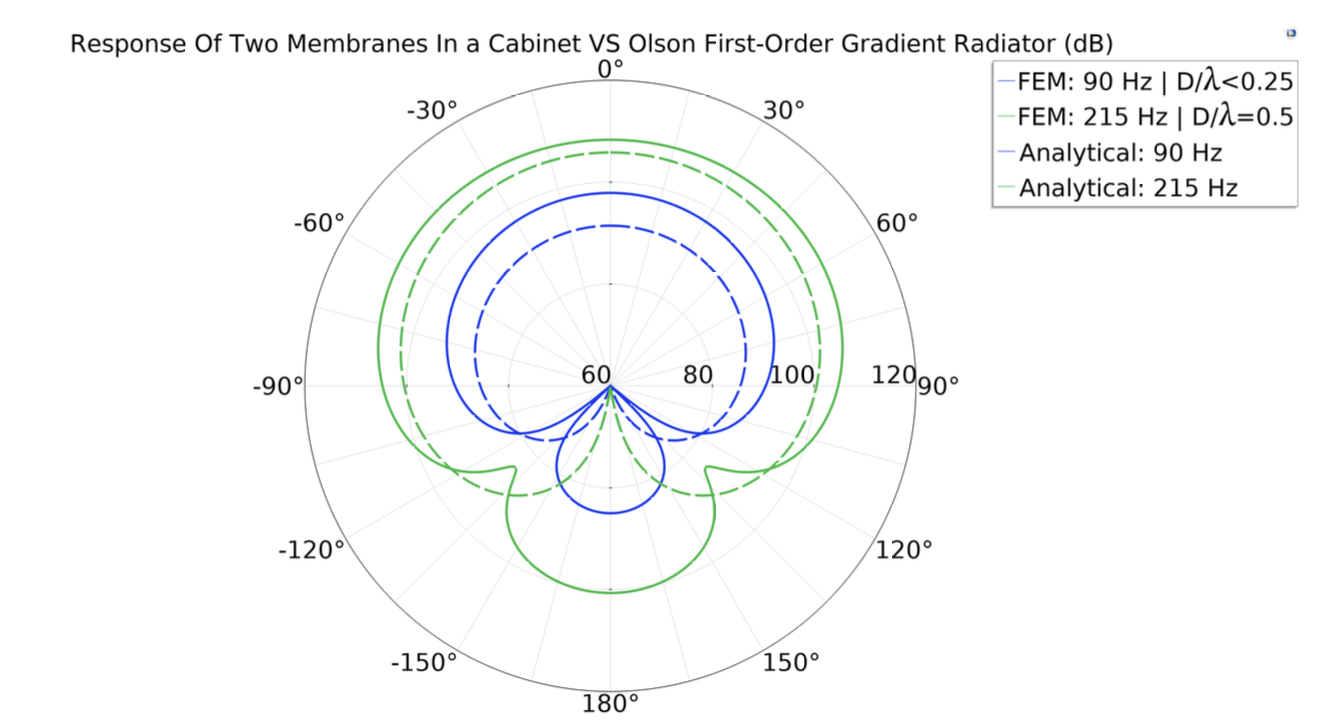
\includegraphics[scale=0.5]{figs/vedierPolar.png}
            \caption{FEM model of the ACL compared with Olson's first order unidirectional loudspeaker.}\cite{vedier}
            \label{vedierPolar}
        \end{figure}

\chapter{Methodology}
    \section{Initial Transfer Function and Directivity Measurement}
        SPEAKER WAS PUT IN THE ANECHOIC
        To build a numerical analysis of the directivity of the axisymmetric loudspeaker system's behavior as a whole over all frequencies, the frequency-domain transfer function of each driver must be measured across the entire X-Y AXIS MAYBE.
        In order to create a precise and accurate measurement free of interference and noise, the drivers were measured, mounted in the loudspeaker unit, in a fully anechoic chamber with a NTi reference-grade measurement mic.
        Ensuring the angle interval of each measurement was consistent, the loudspeaker was mounted to a Four Audio ELF robot arm which rotated the loudspeaker system about the X-Y AXIS MAYBE.
        Swept sine input signals were fed to each driver as the input excitation.
        The two low-frequency drivers were fed by a Samson SERVO-500 power amplifier, whilst the mid-high driver was fed by a University of Salford in-house made mono power amplifier, a 'Dial-a-Watt'.
        The output of the Dial-a-Watt was fed to a KEF-made cross-over, splitting the signal into mid and high frequency bands for the coaxial Uni-Q's mid and high drivers.
        The low frequency drivers had no cross-over filtering applied at this stage of the testing.
        The full signal flow of the transfer function measurement system is shown in Fig.\ref{signalFlow}.
        \begin{figure}[H]
            \centering
            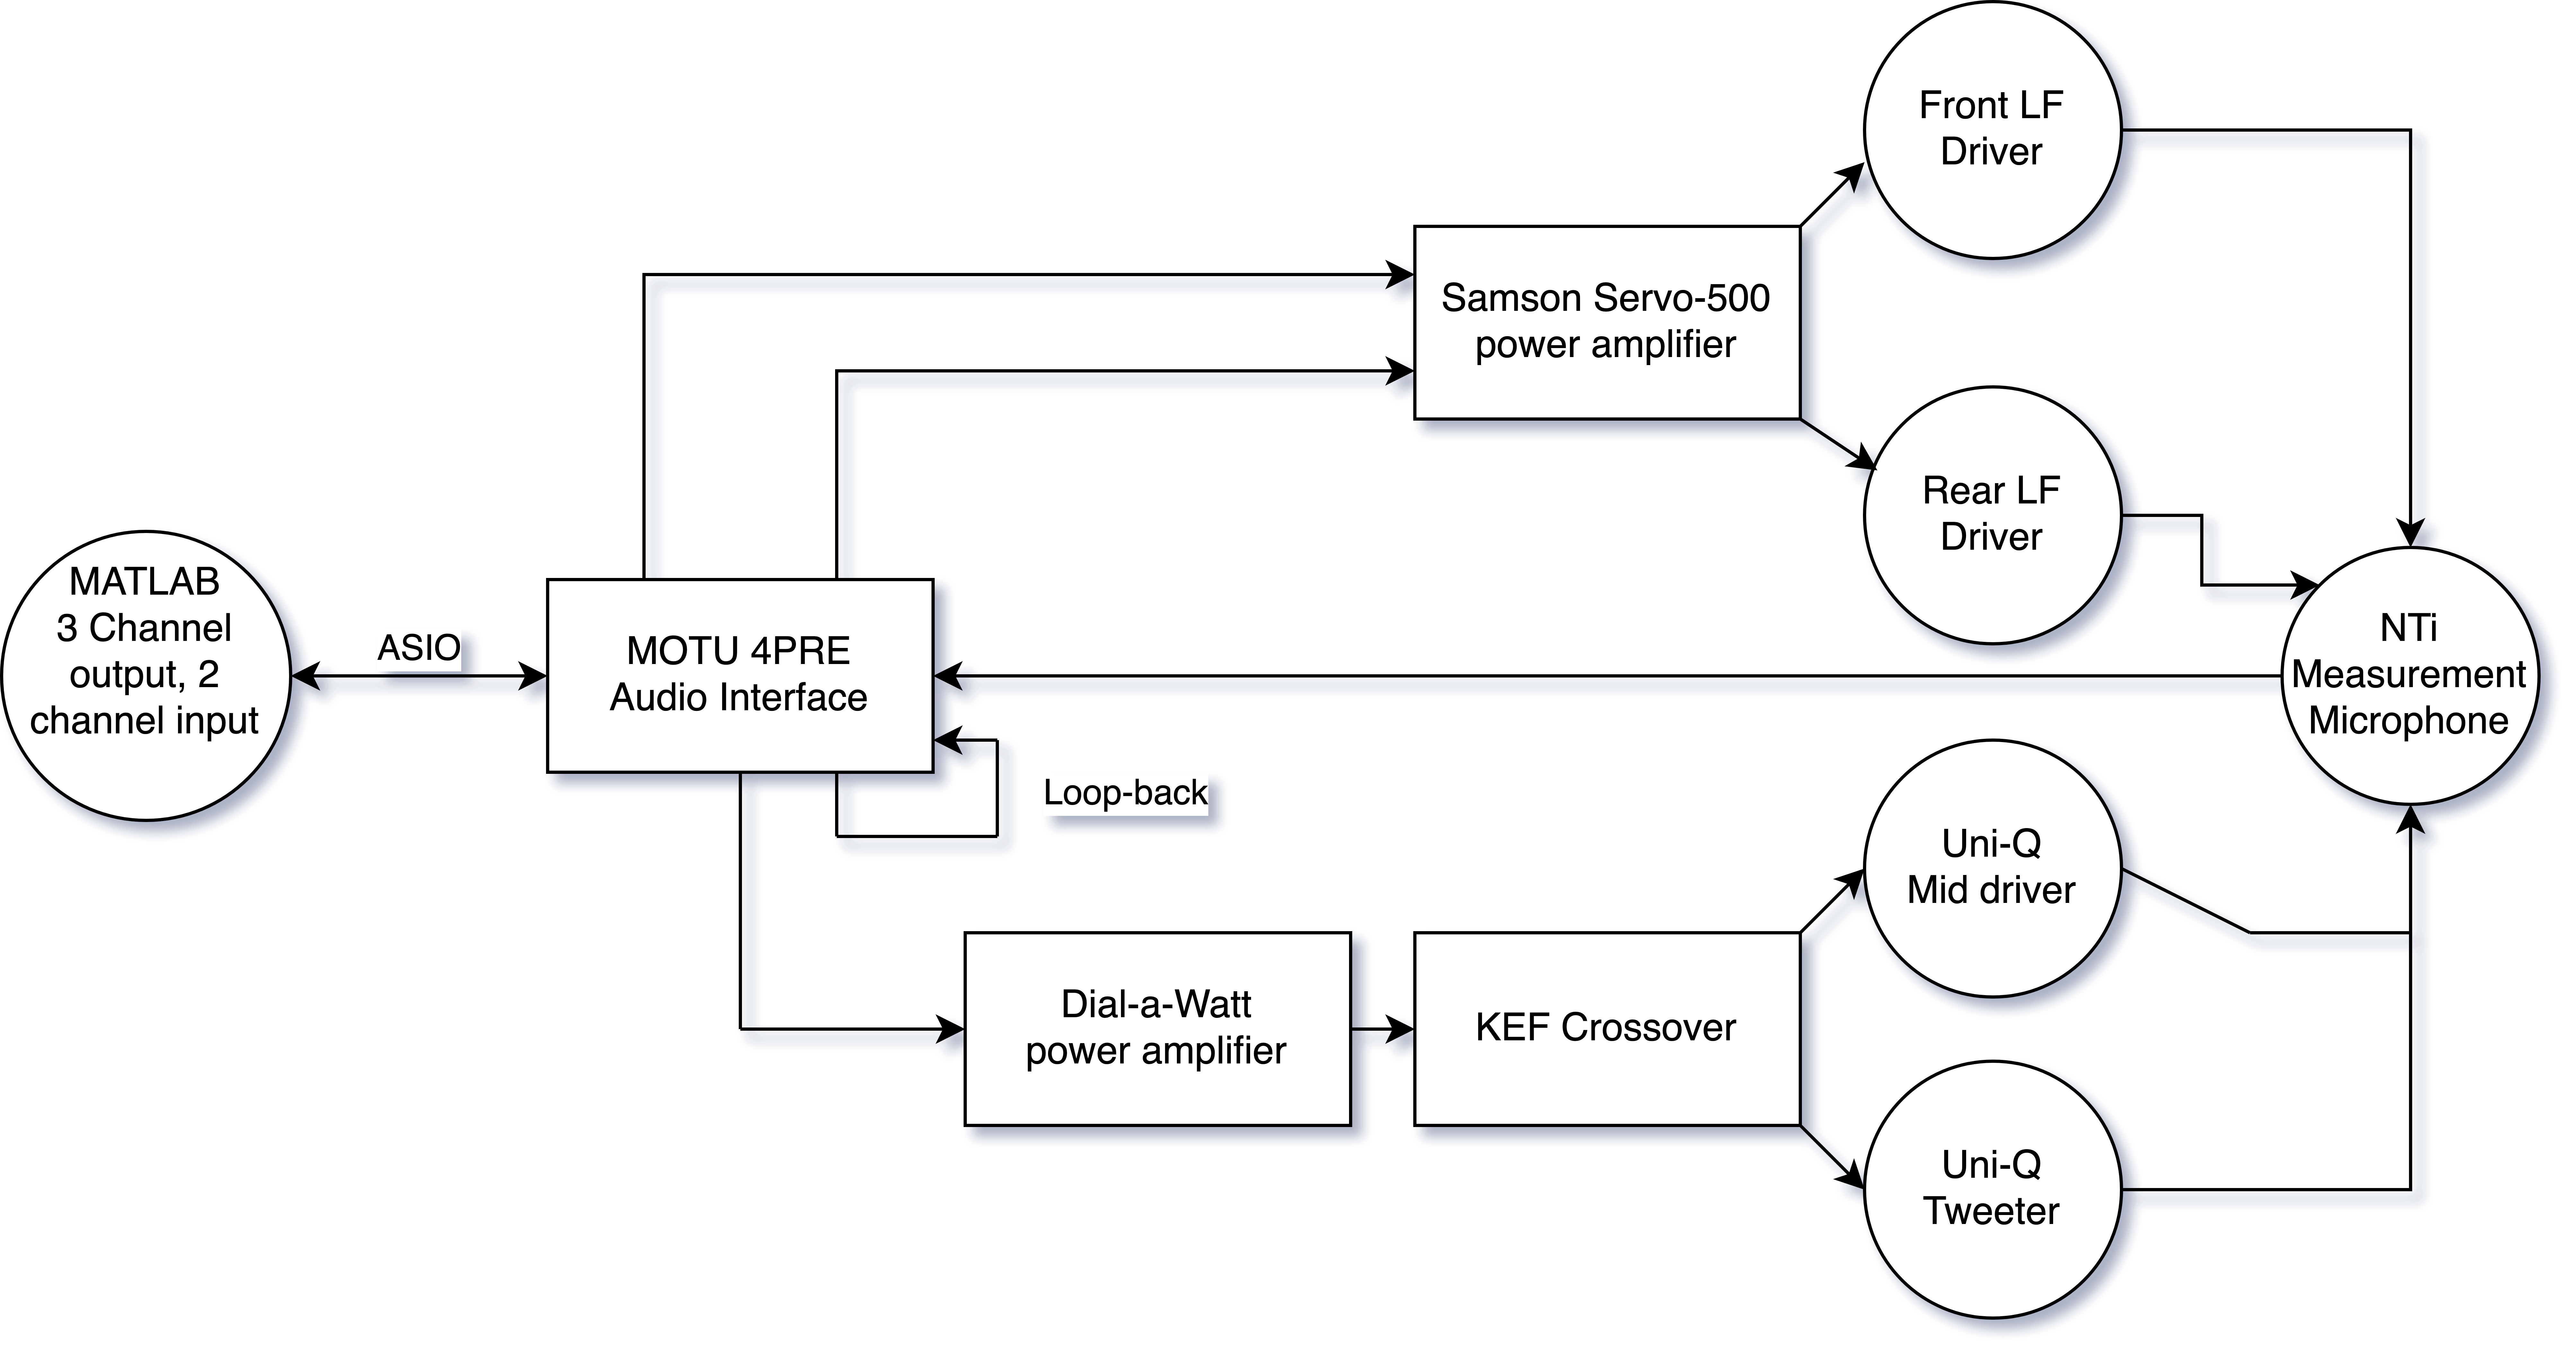
\includegraphics[scale=0.04]{figs/signalFlow.png}%
            \caption{Signal flow of driver transfer function measurement}
            \label{signalFlow}
        \end{figure}

        All audio output, robot arm movements and input recordings were automated through a MATLAB script.
        \begin{figure}[H]
            \centering
            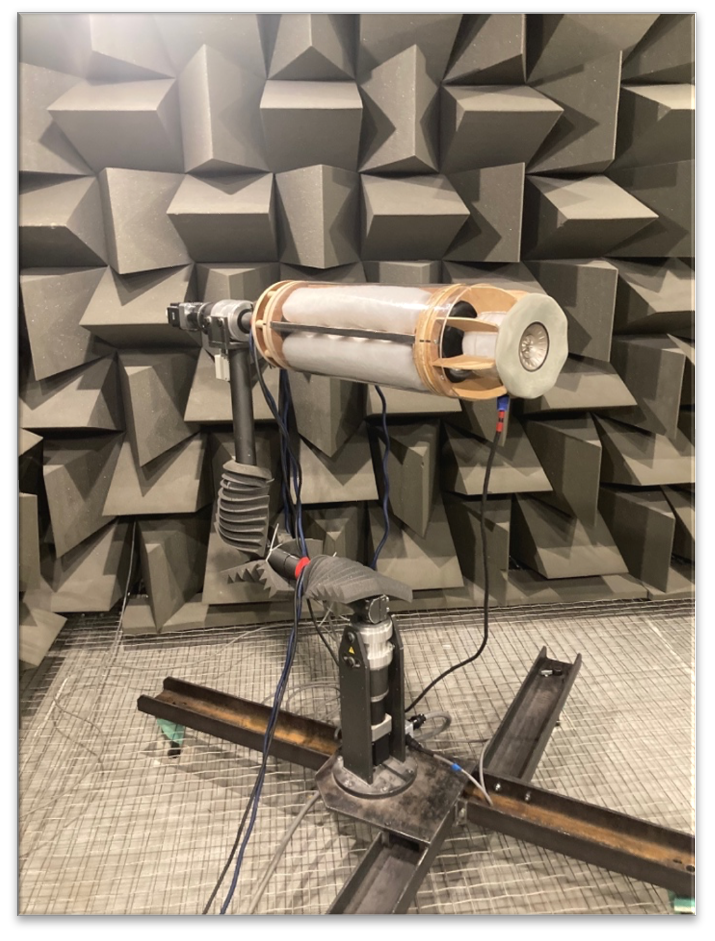
\includegraphics[scale=1]{figs/speakerOnRobot.png}%
            \caption{The prototype loudspeaker mounted for testing in the University of Salford's fully anechoic chamber.}
            \label{speakerOnRobot}
        \end{figure}
        A Bruel \& Kjaer measurement microphone placed 3.6m away was used to record relative sound pressure levels radiating from the loudspeaker drivers for each frequency at 121 angles.

        The raw results from this measurement were immediately processed; the dataset was large in file size and unwieldy to work with in MATLAB, so the data was reduced in size by taking only every 16th frequency point from the original, unnecessarily large frequency resolution.
        This had no apparent affect on the accuracy or validity of the measurements.
        Upon first inspection of the data, anomalous and invalid pressure-over-frequency data was found at a number of angles, shown in Fig.\ref{allAngles}.
        \begin{figure}[H]
            \centering
            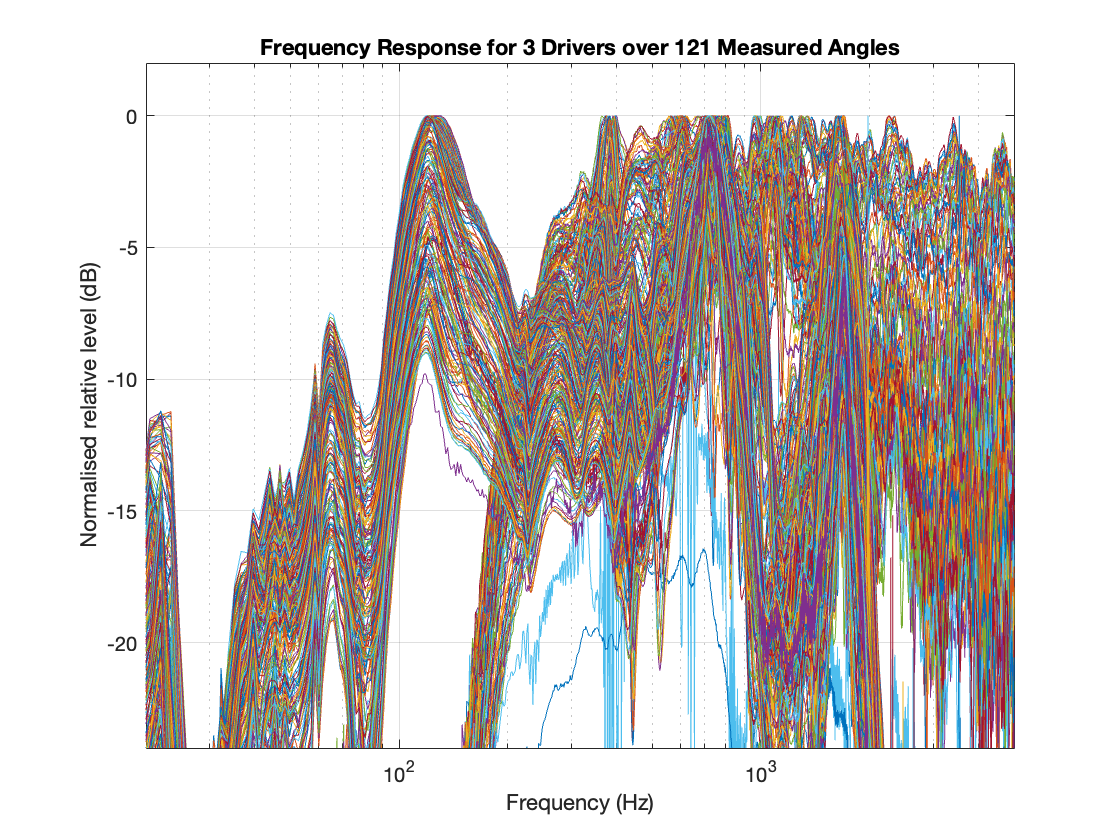
\includegraphics[scale=0.35]{figs/allAngles.png}%
            \caption{Noisy and anomalous data can be seen in the large blue and purple smears to the right. This data needed cleaning.}
            \label{allAngles}
        \end{figure}
        Manually cycling through each angle's driver frequency responses, anomalous data was manually averaged out using it's nearest angle neighbors.

    \section{Rear Driver Correction Filter Design}
        \subsection{Theory}
            The radiation of the rear driver of the ASL needs to have a particular phase and frequency relationship to radiation of the front driver.
            It is important to note that in order to maintain cardioid directivity across all frequencies, the frequency and directivity response of the rear driver in relation to the front driver must be accounted for.

            Using the metric of cardioid directivity given by Jonathan Hargreaves, previously used and elaborated upon in Vedier's paper, a digital filter was used to encourage cardioid directivity across the working frequency range of the LF drivers \cite{vedier}.
            When devising this metric, only the zeroth and first spherical harmonics were considered, as a true cardioid directivity can be described in three dimensions using only these harmonics.
            Incorporating higher order spherical harmonics in to a newer, more precise directivity metric may be useful in a further investigation of the non-cardioid directivity behavior of the ACL, but were beyond the scope of this filter design.
            Vedier's work derives a pair of coefficients $a_0$ and $a_1$ from a more general solution to spherical wave propagation, further stating that if these $a_n$ coefficients are equal, then the radiated pressure waves' directivity must be spherical.
            Using Eq.\ref{a0a1} to find the coefficients $a_0$ and $a_1$ for the front and rear drivers.
            Equation \ref{sphericalPressure}.\ shows how spherical harmonic coefficients can be expressed as a function of pressure over spherical angles, where the $R$ term accounts for any residual directivity.
            \begin{equation}
                p_{ff}(\beta,\alpha) = a_0 + a_1 \cos(\beta) + R(\beta,\alpha)
                \label{sphericalPressure}
                \cite{hargreaves}
            \end{equation}
            \begin{equation}
                \begin{split}
                    a_0(\omega) &= \frac{1}{ikh_0^{(1)}(kr_{meas})} \sqrt{\frac{1}{4\pi}} c_{0,0}(\omega) \\
                    a_1(\omega) &= \frac{1}{ikh_1^{(1)}(kr_{meas})} \sqrt{\frac{3}{4\pi}} c_{0,1}(\omega)
                    \label{a0a1}\cite{hargreaves}
                \end{split}
            \end{equation}
            Equation \ref{a0a1} utilises spherical Hankel functions of the first kind, which are a combination of a Hankel function of the first kind and a spherical Bessel functions of the first and second kind \cite{weisstein}.
            The complex exponential component of the given spherical Hankel function characterizes the outwards propagation and decay of a spherical wave; the negative-signed $-e^{ikt}$ component is in contrast to the rest of the positive-signed complex exponentials in the filter generation script.
            Therefore to keep the complex exponential's signs consistent, the complex conjugate of the defined spherical Hankel functions is taken before their use in any calculations.
            The Hankel functions used are defined in Eq.\ref{hankel}, and are derivatives of those given by Wolfram \cite{weisstein}.
            \begin{equation}
                \begin{split}
                    h_0^1 &= -i  e^{ikr}  \frac{1}{kr} \\
                    h_1^1 &= -e^{ikr}  \frac{kr + i}{kr^2}
                    \label{hankel} \cite{weisstein}
                \end{split}
            \end{equation}

            Conceptually, if the $a_0$ and $a_1$ coefficients are equal, the directivity pattern will be cardioid.
            It should be noted that the response of the $a$ coefficients above 500Hz is mostly irrelevant, as the LF drivers will be filtered out in favour of the Mid-High, which has a favorably cardioid directivity.
            Each driver's $a_0$ and $a_1$ coefficients were derived using the initial frequency and directivity response measurements of the ASL.
            \begin{lstlisting}[style=Matlab-editor, gobble=16]
                function [a0, a1] = Compute_a_coeff(p, beta, k, r)
                    % Hankel functions (spherical bessel functions with decay):
                    h01 = conj(-1i .* exp(1i .* k .* r) .* (1./(k.*r)));
                    h11 = conj(-exp(1i .* k .* r) .* (((k.*r) + 1i)./((k.*r).^2)));

                    % Computing a_0, a_1 coefficients:
                    a0 = (pi./(2i .* k .* h01)) .* mean(p.*sin(beta),2);
                    a1 = ((3.*pi) ./ -(2.*k.*h11)) .* mean(p.*sin(beta).*cos(beta),2);
                
                end
            \end{lstlisting}

            The resulting $a$ coefficients, while precise, were rough in envelope to the point that a closely matching filter would be unfeasible.
            This can be seen when plotting the immediately derived $a$ coefficients, shown in Fig.\ref{acoeffsNoSmooth}.
            \begin{figure}[H]
                \centering
                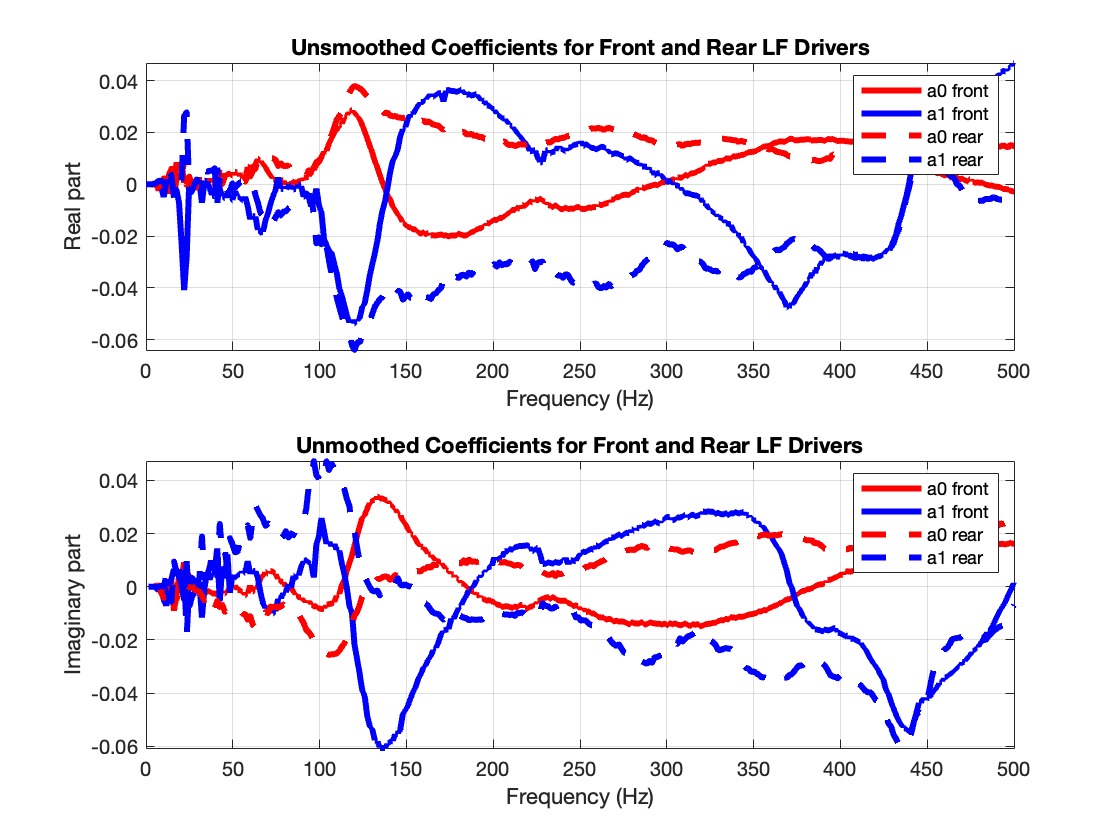
\includegraphics[scale=0.35]{figs/acoeffsNoSmooth.png}%
                \caption{Real and imaginary parts of $a$ coefficients with no smoothing applied.}
                \label{acoeffsNoSmooth}
            \end{figure}
            Figure \ref{acoeffsNoSmooth} plots both the real and imaginary parts of the calculated $a$ coefficients, and in the real and imaginary parts of $a_0$ and $a_1$ for both drivers, the plot is jagged with high dynamic range between 0-150Hz.
            Whilst any frequencies below 20Hz may be disregarded as inconsequential to a human listener, the 20-150Hz range is within the frequency range where the LF drivers are attempting to give a cardioid directivity.
            Thus, any smoothing applied to this region will have the trade-off of reduced precision and accuracy in the ability of the filter to match the $a$ coefficients in this crucial frequency band.
            Finding a good compromise point between the amount post-measurement smoothing and required accuracy in the filter is a point for further study.
            MATLAB's \texttt{smoothdata()} function was used, on it's default setting, to smooth the $a$ coefficients.
            MathWorks describe \texttt{smoothdata()} as a function that: `Returns a moving average of the elements of a vector using a fixed window length that is determined heuristically. The window slides down the length of the vector, computing an average over the elements within each window.' \cite{smoothdata}.
            As the design of the correction filter follows an inverse-FFT methodology, which will be elaborated upon in a further section, only a magnitude response over frequency of the correction filter is needed.
            Therefore, only the magnitude response of the $a$ coefficients was needed to construct the correction filter that makes both $a$ coefficients magnitude equivalent over frequency; this magnitude response can be thought of as an envelope in time without any relevant frequency information, and as such a moving average filter's undesirable frequency characteristics are irrelevant \cite{smith2013digital}.
            Figure \ref{acoeffsSmooth} shows how the moving-average filter has smoothed the $a$ coefficients enough to remove any jagged jumps but keep most of the envelope's main curves and information.
            \begin{figure}[H]
                \centering
                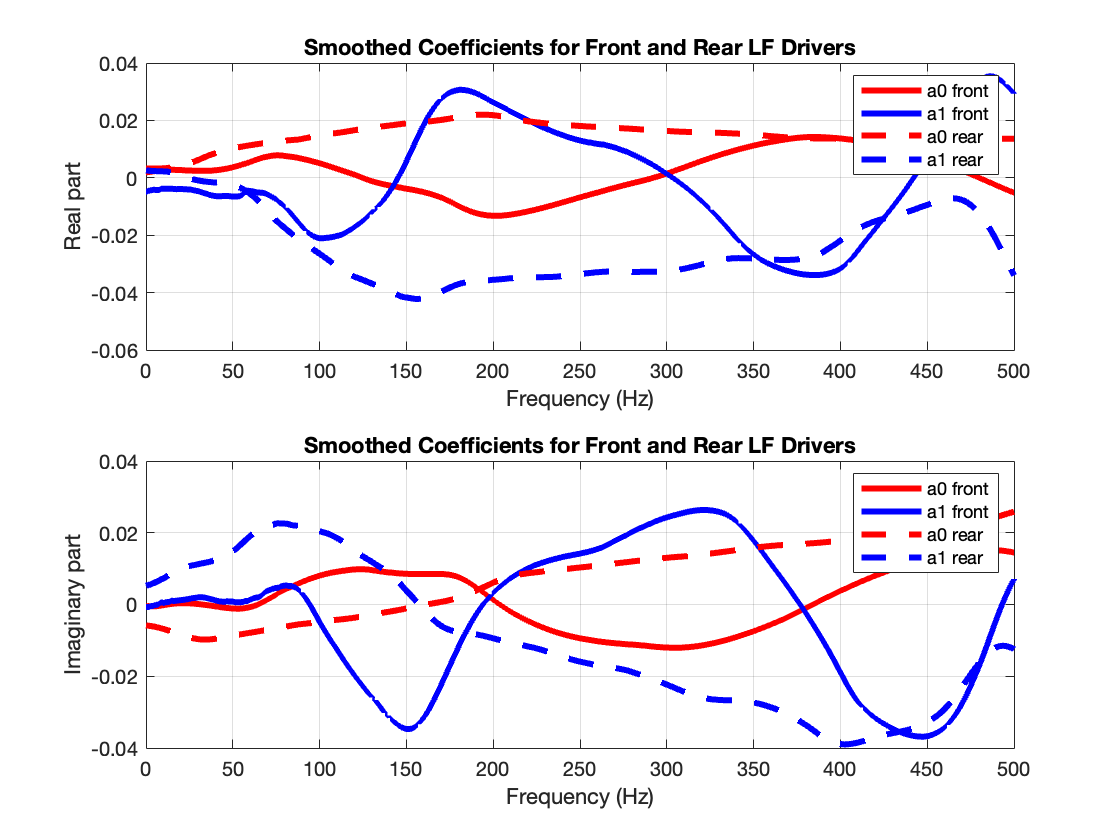
\includegraphics[scale=0.35]{figs/acoeffsSmooth.png}%
                \caption{Real and imaginary parts of $a$ coefficients with smoothing applied.}
                \label{acoeffsSmooth}
            \end{figure}

            The frequency magnitude response of the correction filter was derived by algebraically solving for a hypothetical $\gamma$, the correction filter, across the frequency-domain magnitude of each driver's smoothed $a_0$ and $a_1$ coefficients.
            Equation \ref{gammaAlgebra} shows the magnitude of gamma at each frequency algebraically related to the $a$ coefficients of the front and rear drivers.
            \begin{equation}
                \gamma = \frac{a_{0f} - a_{1f}}{a_{1r} - a_{0r}}
                \label{gammaAlgebra}
            \end{equation}
            Mathematically applying $\gamma$, the derived correction filter, to the rear LF woofer and recalculating the $a_0$ and $a_1$ coefficients for each driver gives a predicted coefficient-over-frequency response shown in Fig.\ref{coeffsPredicted}.
            \begin{figure}[H]
                \centering
                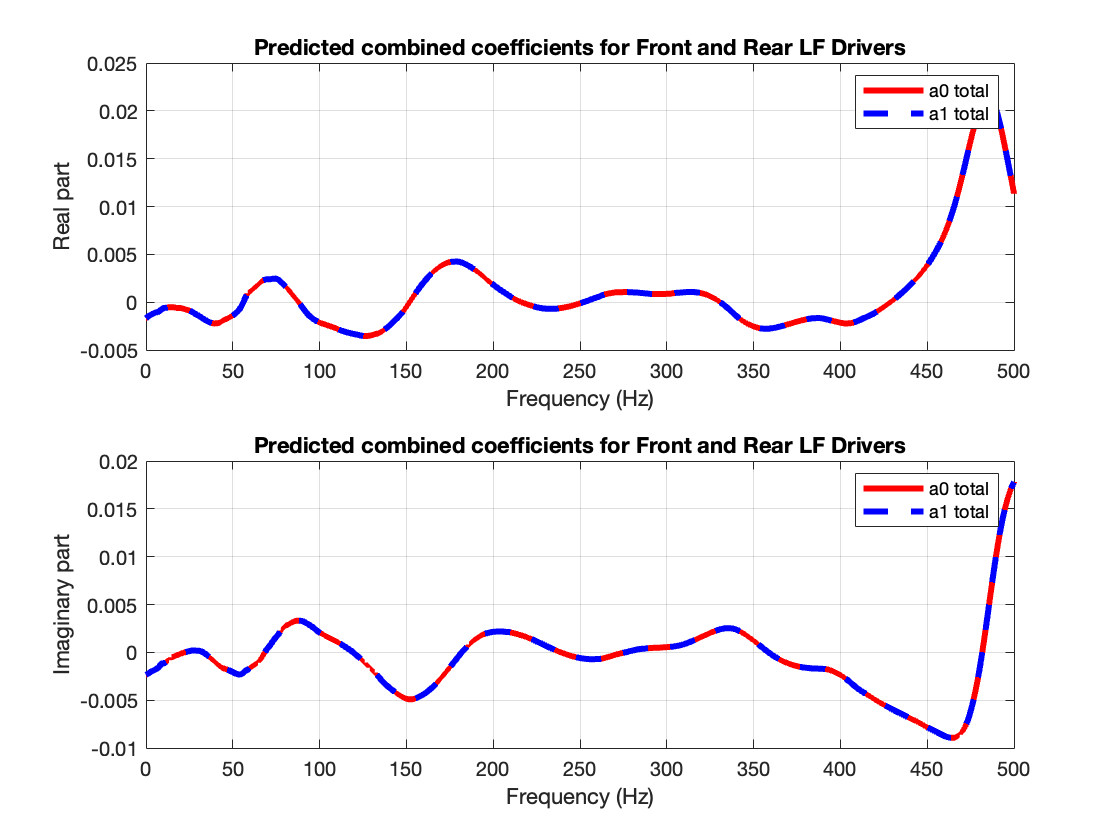
\includegraphics[scale=0.35]{figs/coeffsPredicted.png}%
                \caption{$a_0$ and $a_1$ coefficients remain equal across frequency after $\gamma$ is applied to the measured coefficients.}
                \label{coeffsPredicted}
            \end{figure}
            Whilst the perfectly matching $a_0$ and $a_1$ coefficients shown in Fig. \ref{coeffsPredicted} are promising, and prove the validity of the algebraic derivation $\gamma$, they are ultimately theoretical.
            A plot of the frequency response of $\gamma$ is given in Fig.\ref{gammaMagnitude}.
            Plots of the phase and group delay over frequency of $\gamma$ are given in Fig.\ref{grpDelay}
            \begin{figure}[H]
                \centering
                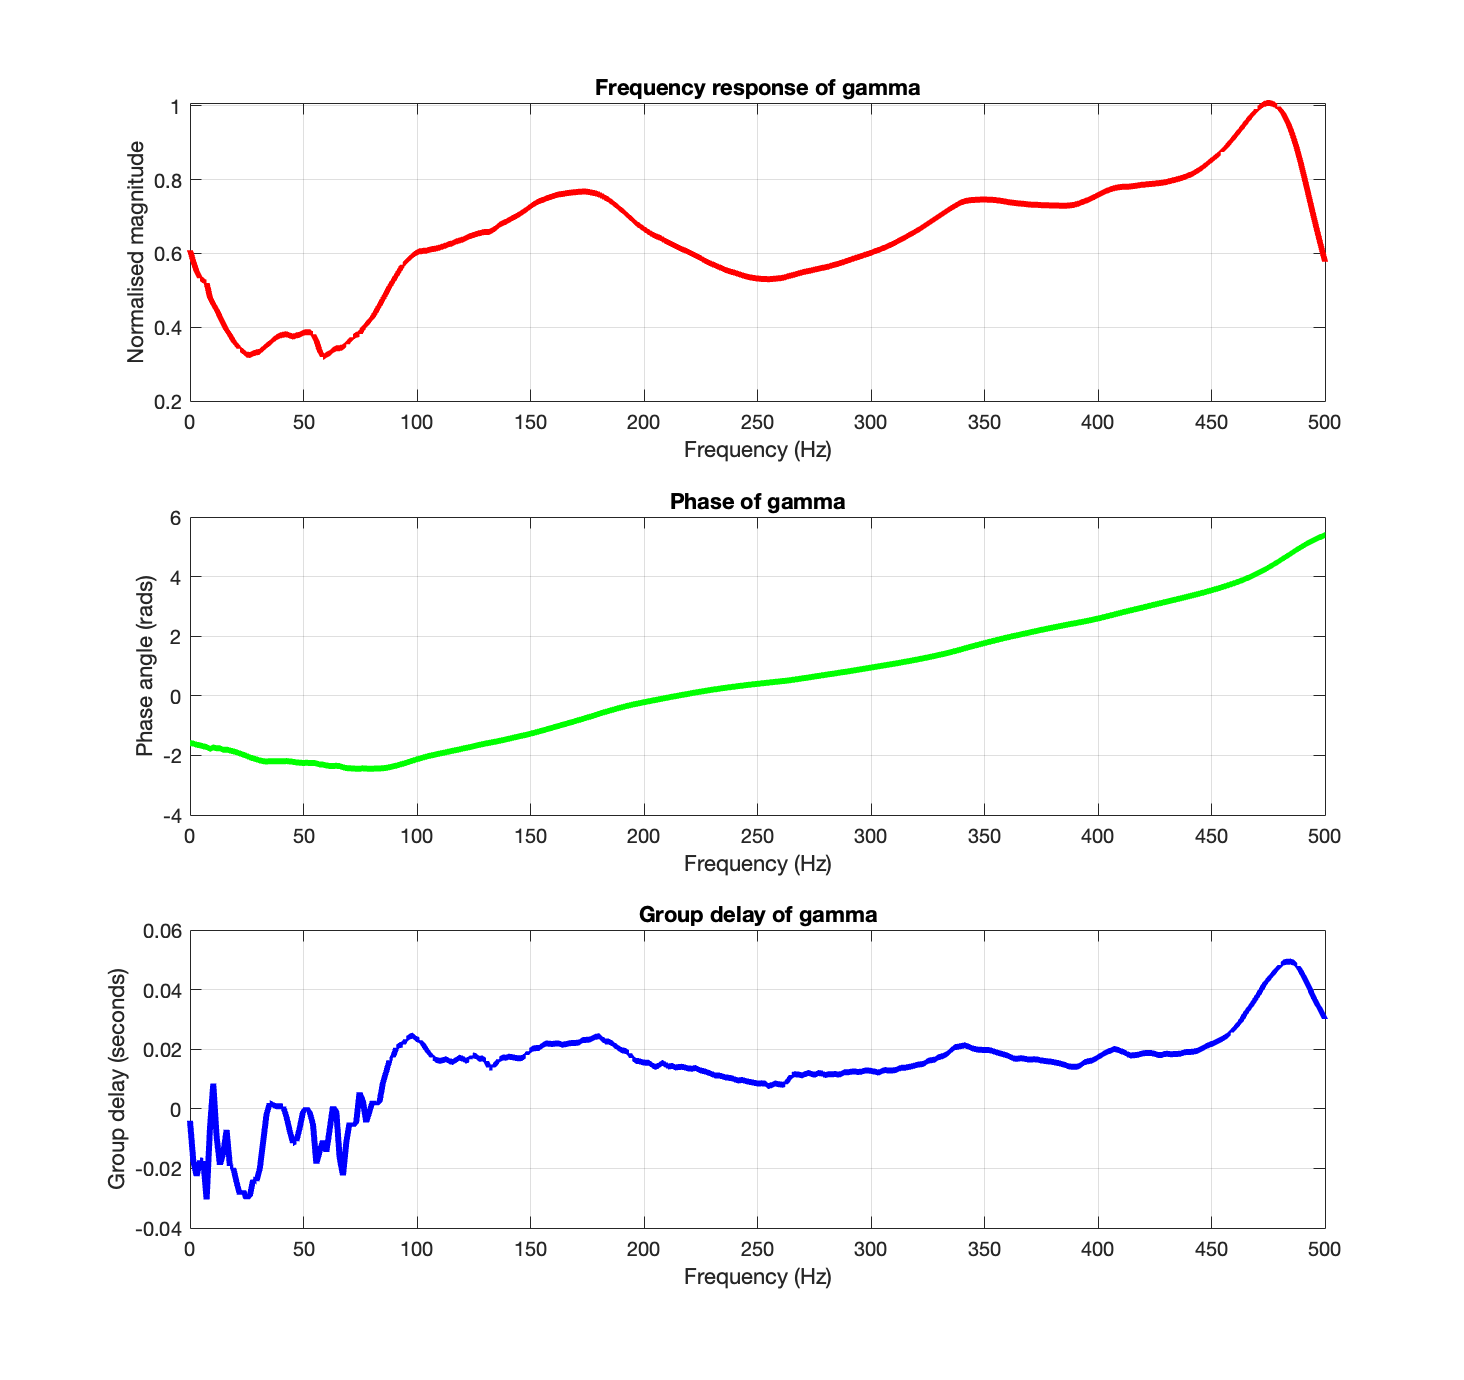
\includegraphics[scale=0.25]{figs/grpDelay.png}%
                \caption{Phase and group delay of the correction filter $\gamma$ are as important as the frequency response.}
                \label{grpDelay}
            \end{figure}
            \begin{figure}[H]
                \centering
                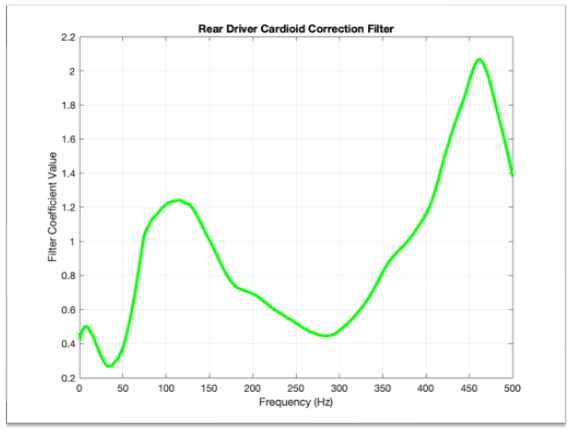
\includegraphics[scale=0.35]{figs/gammaMagnitude.png}%
                \caption{The magnitude of $\gamma$ over frequency.}
                \label{gammaMagnitude}
            \end{figure}
            \begin{figure}[H]
                \centering
                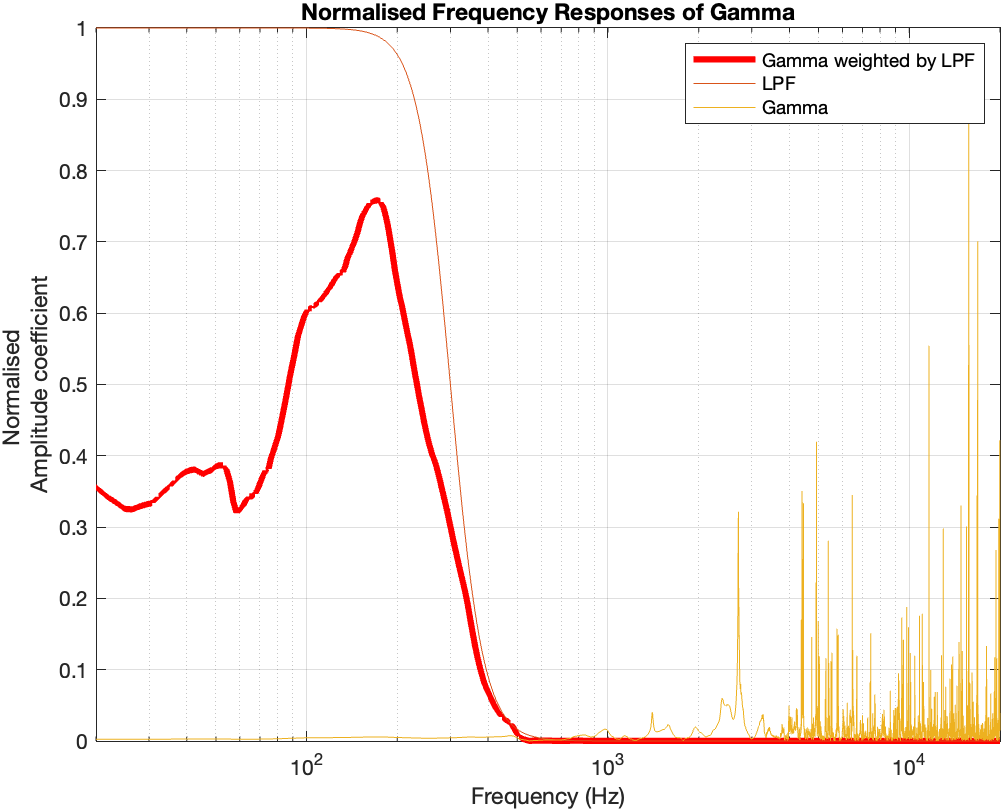
\includegraphics[scale=0.35]{figs/gammaCompare.png}%
                \caption{Normalizing $\gamma$ and plotting over the entire frequency range shows the extent of noise above the relevant frequency range.}
                \label{gammaCompare}
            \end{figure}
            Whilst only the rough range of 20-500Hz is relevant to the LF drivers, the $a$ coefficients and thus $\gamma$ were calculated across the entire frequency range, up to the Nyquist limit, of the measurement system.
            Upon further inspection of the impact of gamma above 500Hz, unwanted noise and dynamic range is found in the filter, shown by the normalized $\gamma$ in Fig.\ref{gammaCompare}.
            The normalized $\gamma$ has such a degree of noise above it's relevant frequency range that the magnitude in the relevant range is almost unnoticeable.
            In order to eliminate this noise, $\gamma$ was weighted with the frequency response of a 4\^{th} order, 300Hz cut-off, Butterworth low-pass filter (LPF).
            Figure \ref{gammaCompare} shows the affect of the LPF on the normalized $\gamma$, all the unwanted noise is removed and the useful frequency range is unchanged, as it remains in the pass-band of the LPF.
            This presents the next challenge: fitting a real-world implementable filter to $\gamma$.

        \subsection{Correction Filter Implementation}
            A simple and direct way to fit an appropriate filter's magnitude response to $\gamma$ is to use the inverse-FFT method, resulting in a finite-impulse response (FIR) filter.
            The inverse-FFT method of FIR filter design uses an inverse-FFT algorithm to compute the time-domain impulse response of a filter from it's frequency-domain magnitude response \cite{li2019digital}.
            As the time-domain impulse response is simply a single finite-length series of scalars, it may be described in the context of FIR filters as a series of $b$ coefficients, where the $a$ coefficients in the in the FIR filter are nonexistent.
            Before taking the inverse-FFT of the $\gamma$ transfer function, it must be weighted (multiplied in the frequency domain) by the LPF.
            Whilst a Butterworth-type frequency response can be manually drawn in MATLAB as an array of weighting coefficients, using MATLAB's \texttt{butter()} function provided easier tweaking of the LPF, as when calling \texttt{butter()}, properties such a filter order can be set.
            MATLAB's \texttt{butter()} generates $a$ and $b$ coefficients of an IIR Butterworth filter, as opposed the FIR desired for $\gamma$.

            Whilst FIR filters are guaranteed, by their finite nature, to decay to zero as stable filters, IIR filters are not, the poles of an IIR filter can lay beyond the unit circle leading to growth instead of decay in the impulse response \cite{litwin2000fir}.
            This can be problematic, and whilst \texttt{butter()}'s design procedure ensures the LPF will be stable the guaranteed stability of FIR filters as opposed to IIR filters was a major factor in choosing to implement $\gamma$ with an FIR filter. 
            It was also important to consider the causality of $\gamma$.
            In DSP, causality refers to the relationship between the input and output signals of a system.
            A causal filter is one in which the output at any given time is dependent only on past and current input values, and not on future input values.
            In other words, the output of a causal filter can only be affected by events that have already occurred, and not by events that will occur in the future.
            Causality is an important concept in digital filters, as it is necessary for filters to be causal in order to be physically realizable.
            For example, if a filter were to rely on future input values to generate its output, it would require knowledge of events that have not yet occurred, which is not possible in a physical system.
            A causal filter can be implemented using a variety of digital filter structures, such as finite impulse response (FIR) filters or infinite impulse response (IIR) filters.
            FIR filters are inherently causal, as they rely only on past and current input values to generate their output.
            IIR filters, on the other hand, may be non-causal, depending on their implementation; it is from this possibility of non-causality that designing an IIR filter to fit the complex magnitude response found in $\gamma$ becomes impractical. 
            One further consequence of causality in digital filters is the existence of phase distortion.
            When a causal filter is applied to a signal, the filter introduces a delay in the output signal relative to the input signal.
            This delay results in a phase shift in the frequency domain, which can cause distortion in the output signal.
            This phase distortion is particularly pronounced in FIR filters, which introduce a linear phase shift that is proportional to the filter's delay.

In summary, causality is a fundamental concept in digital signal processing and is essential for the physical realizability of digital filters. Causal filters only rely on past and current input values to generate their output, which ensures that they do not require knowledge of future events. However, the introduction of delay in causal filters can result in phase distortion, which can affect the quality of the output signal.

            After the Butterworth LPF was generated, MATLAB's in-built texttt\ {freqz()} function was used to convert the LPF's $a$ and $b$ filter coefficients into a frequency-domain transfer function.

            From here, the frequency-domain transfer function of the LPF was multiplied with the frequency-domain transfer function of $\gamma$, giving the weighted $\gamma$ frequency response shown in Fig.\ref{gammaCompare}.
            This simple multiplication in the frequency domain should produce no inconsistencies or invalidity of the resultant filter; multiplication in the frequency domain is the same as convolution in the time domain \cite{stanfordConvolution}.
            All that was left from this point was to transform the new, weighted $\gamma$ into it's impulse response using an inverse FFT, such that the time-domain effects of the filter can be further investigated.
            \\
            As aforementioned, the inverse-FFT method of FIR filter design was ultimately used to generate a working $\gamma$ rear-driver correction filter.
            Using MATLAB's in-built \texttt{ifft()} function requires some considerations: The convolution is CIRCULAR NOT CIRCULAR PROS AND CONS.

            The impulse response of a finite impulse response (FIR) filter is the sequence of filter coefficients that, when convolved with an input signal, produces the filter's output signal.
            The length of the impulse response corresponds to the number of filter taps, which determines the filter's order. In an FIR filter, the impulse response is finite, meaning that it has a fixed length and eventually decays to zero.
            One important characteristic of FIR filters is that the impulse response is always causal, meaning that the output of the filter at any given time depends only on past and current input values, and not on future input values. As a consequence of this causality, the impulse response of an FIR filter cannot extend infinitely into the past.
            However, the impulse response of an FIR filter can extend infinitely into the future, or more precisely, it can wrap around from the end of the sequence to the beginning. This is known as circular convolution, and it occurs when the input signal is periodic. In other words, if the input signal repeats itself every N samples, then the convolution of the input signal with the filter impulse response will also repeat itself every N samples.
            The concept of circular convolution is important in FIR filter design, as it allows us to treat the impulse response of an FIR filter as a circular buffer. This means that we can implement the filter using a delay line with N samples, where N is the length of the impulse response. The delay line holds the N most recent input samples, and the filter coefficients are applied to the samples in the delay line using circular indexing. This circular indexing ensures that the impulse response "wraps around" from the end to the beginning of the delay line, enabling us to implement the filter with a fixed number of multiply-accumulate operations per sample.
            In summary, the impulse response of an FIR filter can "wrap around" from the end to the beginning, allowing us to implement the filter using circular convolution. This concept is important in FIR filter design, as it enables us to implement the filter with a fixed number of multiply-accumulate operations per sample, regardless of the length of the filter

            
            COMPARE PHASE GRPAHS TO OLSONS PHASE GRAPHS (FIG 3)
            Olson:
            delay is given as d/2 and kD/2 makes the expression frequency dependent.
            short delay gives wide enough comb filtering such that u get 2 bumps like in olsons fig 3.


            


            The generated impulse response, shown in Fig., is non-causal, with a substantial section wrapped back around $t=0$ to the end of the response.
            This generated audible artifacts and ringing when convolved with any audio signal and played back.
            Thus, the impulse response of the filter was processed to eliminate this non-causality, but preserve it's original frequency and phase characteristics.
            Using MATLAB's \texttt(tukeywin()) function, a window tending zero at it's stop bands was used to keep the useful section of the impulse response and discard the `tail' of the impulse response.
            A brief investigation into the relationship between the width of the window and the error between the windowed impulse response's frequency response and the original impulse response's frequency response was carried out.

            Certain interactions between the front ad rear drivers will require the rear driver



    \section{Measurement Revisited, Post Filtering}


\chapter{Discussion and Conclusions}

\chapter{Further Work}
    A-coeff smoothing investigation.
    Driver model suitability
    length of coupled chamber
    cavity resonances ala KEF

\bibliographystyle{IEEEtran}
\bibliography{theBib.bib}

\end{document}


